\documentclass[]{article}
\usepackage{amsmath}
\usepackage{amsfonts}
\usepackage{amssymb}
\usepackage{algorithmic}
\usepackage{algorithm}
\usepackage{tikz}
\usepackage{graphicx}
\usepackage{mdframed}
\usepackage{paralist}
\usepackage{listings}

\definecolor{dkgreen}{rgb}{0,0.6,0}
\definecolor{gray}{rgb}{0.5,0.5,0.5}

\lstset{
  language=Python,
  breaklines=true,
  showstringspaces=false,
  frame=single,
  aboveskip=3mm,
  belowskip=3mm,
  columns=flexible,
  basicstyle={\small\ttfamily},
  numbers=none,
  numberstyle=\tiny\color{gray},
  keywordstyle=\color{blue},
  commentstyle=\color{gray},
  stringstyle=\color{dkgreen},
  breakatwhitespace=true,
  tabsize=3
}

\title{CAGD - Homework 2}
\author{Josefine St{\aa}l \& Erik Ackzell}

\begin{document}

\maketitle
\section*{Task 1}
In this task we implement subdivision to split a B\'ezier curve into two different B\'ezier curves. This is implemented as a method of a Python class, see Appendix 1. Details can be seen in the code. We then test our code by defining a B\'ezier curve with control points $(-1, 0), (0, 1), (2, 0)$, subdividing at $t=0.4$. In our test, the control points of the two new B\'ezier curves were $(-1, 0), (-0.6, 0.4), (-0.04, 0.48)$ and $(-0.04, 0.48), (0.8, 0.6), (2, 0)$. The original curve can be seen in the figure below.
\begin{figure}[h!]
	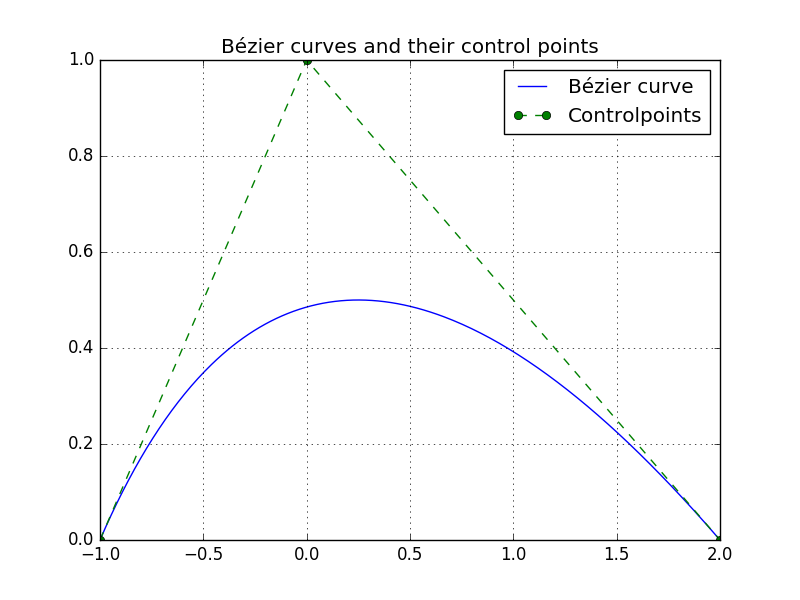
\includegraphics[scale=0.6]{beziercurvefig}
\end{figure}

\section*{Task 2}
In this task we implement degree elevation for the B\'ezier curve with the same control points as in task 1. This is implemented as a method of a Python class, see Appendix 1. Details can be seen in the code. In our test, the control points of the B\'ezier curve from task 1 were used, and the degree was increased to four. The control points of the new curve were $(-1, 0), (-0.5, 0.5), (0.17, 0.7), (1, 0.5), (2, 0)$.

\section*{Task 3}
In this task, we used the trivial reject approach in order to determine the intersection of a B\'ezier curve and a line. This is implemented as a method of a Python class along with a rectangle class and a line class, see Appendix 1. Details can be seen in the code. In our test, we used the B\'ezier curve with control points $(0, 0), (9, -4), (7, 5), (2, -4)$ and the line passing through $(4, 5)$ and $(6, -4)$. The intersections found were $(5.32, -0.94)$ and $(5.13, -0.10)$.

\section*{Task 4}
Let $b$ and $c$ be two B\'ezier curves with domain $[0,\frac{1}{3}]$ and $[\frac{2}{3},1]$ respectively with control points $\{b_0,b_1,...,b_n\}$ and $\{c_0,c_1,...,c_m\}$. B\'ezier curves are always polynomial curves and hence also $C^\infty$. The question is what is required for the composite of the two curves to be $C^1$ or just $G^1$? For a curve to be $C^1$, $C^0$ must be satisfied to start with. The continuity of the curve is satisfied when $b_m=c_0$. A part from continuity, the curves must be collinear in the meeting point. That is that the tangent at the meeting point, including the points  $b_{m-1}$, $b_m=c_0$ and $c_1$, is continuous. Finally the derivative at the meeting point must be continuous.

For $G^1$ on the other hand, the derivatives must not be equal, it is enough for the derivatives to have the same directions. The collinearity must still be fullfilled.

In our case with the two curves $b$ and $c$ we can observe the two domains which do not overlap. Hence it is impossible for $b_n$ and $c_0$ to coincide. Therefore we can not have either $C^1$ or $G^1$ for the composite of the two curves.

\section*{Task 5}
A basis is invariant under affine domain transformations if the basis functions remains unchanged after applying the affine map $\phi:[a,b] \rightarrow [0,1]$ with $$\phi(u)=\frac{u-a}{b-a}$$
B\'ezier polynomials are invariant under affine domain transformations, let us check if the Monomial and/or the Lagrange basis are invariant as well.

Let $C(x)=\sum_{i=0}^{n}c_ix^i$ and $D(x)=\sum_{i=0}^{n}d_ix^i$ be two functions of Monomial form. Then, $$\alpha C(x) + (1-\alpha)D(x)=\alpha\sum_{i=0}^{n}c_ix^i + (1-\alpha)\sum_{i=0}^{n}d_ix^i$$
With $n$ being finite we have,
$$=\sum_{i=0}^{n}[\alpha c_i+(1-\alpha)d_i]x_i\hspace{1cm}\square$$ \\
\\
Hence, the monomial form is invariant under affine domain tranformations. 

Now let the basis functions be the Lagrange polynomials $$L_i^n(x)=\prod_{j=0, j\neq i}^{n}\frac{x-x_j}{x_i-x_j}$$ and $C(x)=\sum_{i=0}^{n}c_iL_i^n$ and $D(x)=\sum_{i=0}^{n}d_iL_i^n$. With the same reasoning as above we can show that 
$$\alpha C(x) + (1-\alpha)D(x)=\sum_{i=0}^{n}[\alpha c_i+(1-\alpha)d_i]L_i^n(x)$$
and the Lagrange form is indeed invariant under affine domain transformations. $\square$

\section*{Task 6}
In this task, we change the appearance of a curve (top curve in figure below to the lower curve) by first applying a degree elevation followed by modifying the control points. It is clear that the lower curve can not be a quadratic curve due to its s-shape, that is why the degree elevation is needed. The control points of the original curve is given by $(0, 0), (1, 1), (2, 1)$ and the second curve has control points $(0, 0), (0.25, 0.05), (1, 1), (2, 1)$.

\newpage
\begin{figure}[h!]
	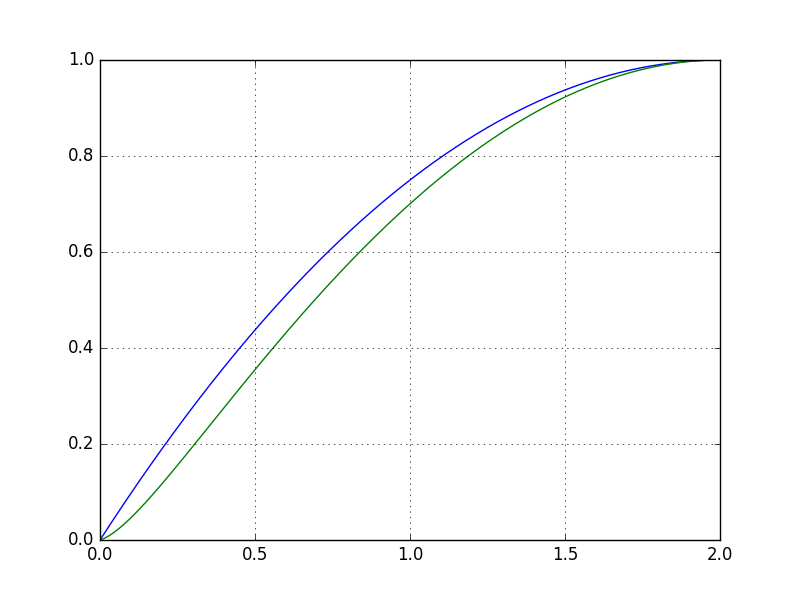
\includegraphics[scale=0.6]{non_symmetric_degree_elevation}
\end{figure}


\newpage
\section*{Appendix I}
Code for task 1-3.
\lstinputlisting[lastline=347]{beziercurveclass.py}

\end{document}
